\chapter{Idémyldring}
I dette steget i prosessen er målet å generere en liste over det vi tror kan være mulige årsaker til problemet. Det er en del forskjellige verktøy en kan bruke for å oppnå dette, men vi har valgt å benytte Idémyldring på basis av RCA boken \cite{RCA} sin fremgangsmåte for valg av verktøy, og på bakgrunn av vår tidligere kunnskap om hvordan brukere vanligvis kompromitteres. 

\section{Idémyldring}
I rotårsaksanalyse finnes det to ulike måter å gjennomføre Idémyldring på, Strukturert- og Ustrukturert Idémyldring. I den strukturerte versjonen får hver deltaker sin tur til å komme med en idé, og dette sikrer at alle får delta like mye. På den ustrukturerte måten kan alle komme med idéer når de dukker opp, og fungerer mye mer spontant enn den strukturelle. Det er spesielt viktig å ikke omformulere eller diskutere forslagene etterhvert som de kommer, dette skal gjøres etter Idémyldringsøkten er over.

\subsection{Ønsket utbytte}
Ønsket utbytte ved å bruke idémyldring var for å få en forståelse av hva som kan være rotårsaken til at ansatte sine kontoer blir kompromittert, og hvordan passord og brukernavn kan komme på avveie.

\subsection{Gjennomførelse}
Det første som ble gjort når økten startet var å kommunisere og skrive opp problemstillingen på en tavle. Vi valgte å strukturere Idémyldringen som et tankekart ettersom dette var en kjent løsning for gruppen, og brukte den ustrukturerte tilnærmingen til Idémyldringen på grunn av dens uformelle struktur, og fordi vi som en gruppe alle tør å komme med innspill. Hvis folk ikke hadde turt å komme med innspill, så hadde vi heller ha gått over til å bruke skriftlig idémyldring. 

Vi diskuterte og prøvde å komme med mulige måter folk kan kompromittere brukerkontoer til de ansatte ved skolen, og hvordan passord og brukernavn kan komme på avveie.

\subsection{Resultater}
Etter øktene var ferdig ble det gjort en vurdering av resultatene og de ble kategorisert i henhold til likhetstrekk, under en fellesnevner som for eksempel sosial manipulering. Resultater og gruppering er som vist i figur \ref{fig:idemyldring} under.

\begin{figure}[H]
    \centering
    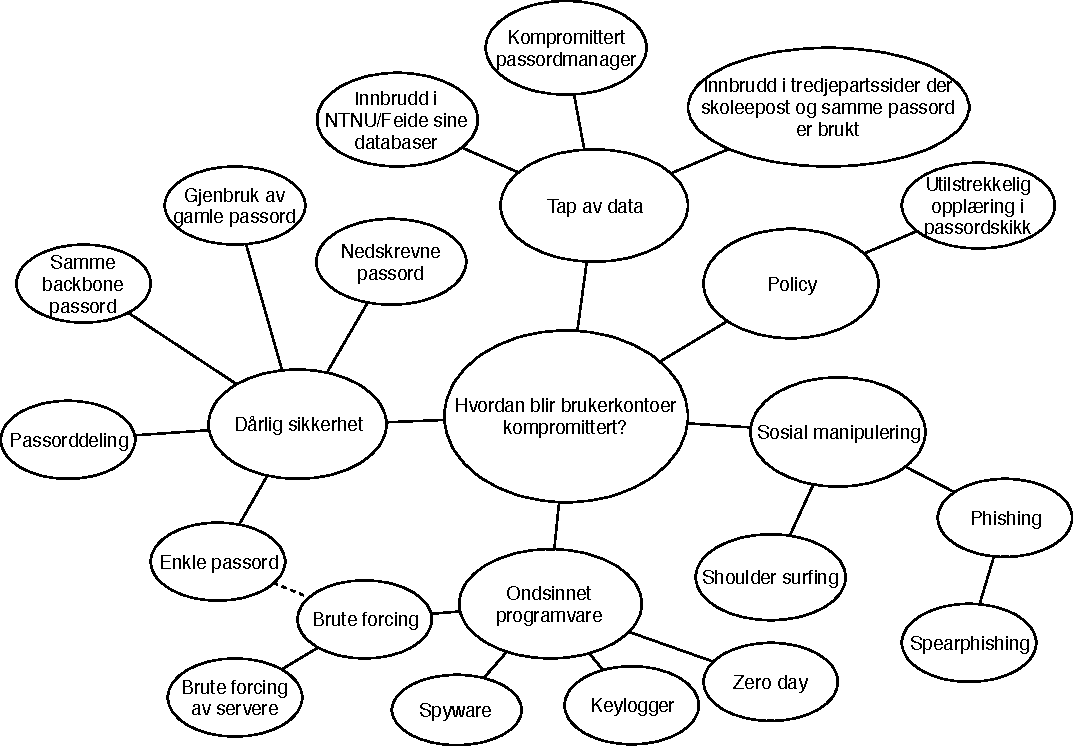
\includegraphics[scale=0.5]{case_2/bilder/idemyldring.pdf}
    \caption[Idémyldring]{Resultater og gruppering av idémyldringen}
    \label{fig:idemyldring}
\end{figure}

Resultatene er gruppert inn i 4 hovedkategorier:
\begin{description}
    \item [Dårlig sikkerhet] her er alt fra for enkle passord til passordgjenbruk.
    \item [Tap av data] sider som dropbox har en lekkasje av brukere.
    \item [Sosial manipulering] hvordan man kan få informasjon/tilgang ved å lure noen.
    \item [Ondsinnet programvare] programvare, brukt som hjelpemiddel for å få tak i brukerinformasjon.
\end{description}

\subsection{Konklusjon av verktøyet}
Dette var et effektivt verktøy for å få en overordnet oversikt over hva årsakene til at brukerkontoer blir kompromittert og grunner til at passord og brukernavn kan være på avveie. Verktøyet fungerte godt til å komme med mulige måter for aktører å få tilgang til brukerkontoer, eneste som trekker tilbake er det at vi ikke har fått et godt bilde av hvorfor angripere velger å gå etter ansattkontoer, selv om vi fikk et litt simpelt bilde på dette med problemforståelsen.
